\documentclass[border=4pt]{standalone}
\usepackage[T1]{fontenc}
\usepackage{helvet}
\renewcommand{\familydefault}{\sfdefault}
\usepackage{graphicx}
\usepackage{caption}
\usepackage{amsmath}
\captionsetup{font={sf,footnotesize},labelfont={sf,bf,footnotesize},justification=justified,singlelinecheck=false}
\begin{document}
\setcounter{figure}{9}
\begin{minipage}{7.20in}
\centering
\begin{figure}[htbp]
    \centering
    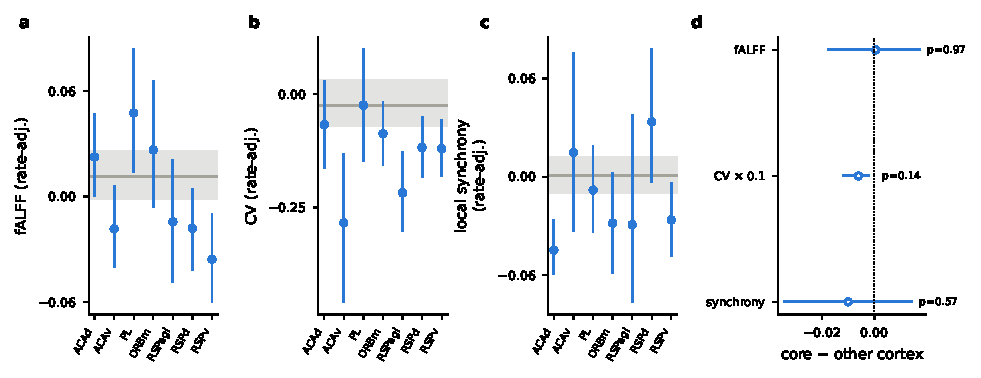
\includegraphics[width=\linewidth]{fig10_single_region_panels.pdf}
    \caption{\textbf{a} Single-region resting metrics of the grey screen for each core region: fALFF per neuron (fraction of 0.01--0.1 Hz power in the 1 s binned rate after regressing wheel, licks and motion energy, residualised on log firing rate), mean over mice with 95\% bootstrap CI. Grey line and band: all other cortex. \textbf{b} Fluctuation amplitude (coefficient of variation of the 1 s rate, rate-adjusted). \textbf{c} Local synchrony (ReHo analogue): mean pairwise correlation between neurons of a region on one probe in still 1 s bins, rate-adjusted. \textbf{d} Core minus other cortex for the three metrics: 95\% mouse-bootstrap CI and region-permutation p (open markers: p $\geq$ 0.05).}
    \label{fig:grey_single}
\end{figure}
\end{minipage}
\end{document}
